The system was built in steps, and each step depends on the one before it: building the dataset, measuring what the laptop could handle, choosing and training the models, delivering an offline runtime, and finally evaluating both models once. Table~\ref{tab:milestone-summary} lists those steps and what each one produced, and Figure~\ref{fig:system-overview} shows how the parts fit together.

\begin{table}[H]
\centering
\small
\renewcommand{\arraystretch}{1.22}
\begin{tabular}{L{3.1cm}L{6.2cm}L{4.7cm}}
\toprule
\textbf{Implemented component} & \textbf{Contribution} & \textbf{Verified outcome} \\
\midrule
Dataset construction & Repairing broken messages without losing which article they came from, removing duplicates, checking that every highlighted phrase appears in the text, limiting how much any one article contributes, and keeping messages from the same article in one set & 2{,}097 messages; 1{,}658/219/220; no article appears in two sets \\
Quality checking & Automatic scoring of every message by a judge model, 100 messages checked by hand across all four classes, and 324 doubtful labels reviewed and corrected one by one & 66.52\% pass the judge; 44/100 pass the manual check; the two agree on 87/100 \\
Hardware decision & Short LoRA and NF4-QLoRA test runs on the same laptop, before committing to either & QLoRA chosen: 395~MiB of video memory left free against 9~MiB for LoRA, and neither ran out of memory \\
Qwen adaptation & Three epochs, 1{,}245 steps, trained locally with QLoRA, with a strict required output format the model had to follow & Validation macro F1 0.988515; checkpoint 200 \\
PhoBERT baseline & Fresh three-epoch, 312-step full Vietnamese classification-head training & Validation macro F1 0.984893; checkpoint 100 \\
Portable model file & The trained Qwen adapter merged into its base model and converted to Q8\_0 & A 4{,}280{,}403{,}232-byte GGUF file, loaded and checked twice \\
Final evaluation & Both finished models run once, on the same 220 held-out messages & Macro F1: Qwen 0.980493, PhoBERT 0.990892 \\
Records kept & Full training logs, loss curves, raw predictions, the exported model, a record of what failed along the way, and a correction about file access & Every number in this report can be traced back to the file that produced it \\
\bottomrule
\end{tabular}
\caption{Implemented project contributions and the strongest verified outcome for each.}
\label{tab:milestone-summary}
\end{table}

\begin{figure}[H]
\centering
\begin{tikzpicture}[
  % every box gets the SAME fixed width and height, so a box with three lines of
  % text cannot grow upwards into the header band above it
  obox/.style={draw=CVBLUE!70!black, fill=CVBLUE!10, rectangle, rounded corners=3pt,
    text width=2.0cm, minimum height=1.60cm,
    align=center, font=\small, inner sep=4pt},
  rbox/.style={draw=black!55, fill=black!5, rectangle, rounded corners=3pt,
    text width=2.0cm, minimum height=1.60cm,
    align=center, font=\small, inner sep=4pt},
  ohdr/.style={draw=CVBLUE!80!black, fill=CVBLUE, rectangle, rounded corners=4pt,
    minimum width=14.6cm, minimum height=0.52cm,
    align=left, font=\small\bfseries, text=white, inner sep=6pt},
  rhdr/.style={draw=black!70, fill=black!70, rectangle, rounded corners=4pt,
    minimum width=14.6cm, minimum height=0.52cm,
    align=left, font=\small\bfseries, text=white, inner sep=6pt},
  arr/.style={-{Stealth[length=2.7mm,width=2.1mm]}, line width=0.9pt,
    CVBLUE!70!black, shorten >=1pt, shorten <=1pt},
  darr/.style={-{Stealth[length=2.7mm,width=2.1mm]}, line width=0.9pt, dashed,
    dash pattern=on 3pt off 2.5pt, black!50},
]

%% ── Handoff drawn FIRST, so the runtime header band paints over the middle of
%%    it and the line reads as passing behind the band rather than through the
%%    title text. It re-emerges just above the box it feeds. ─────────────────
\draw[darr]
  (6.10,-2.05) -- (6.10,-2.50)
  -- node[above, pos=0.62, font=\scriptsize, text=black!60] {trained model files}
  (0.00,-2.50)
  -- (0.00,-3.60);

%% ── Section headers ──────────────────────────────────────────────────────────
\node[ohdr] at (0,  0.00) {(1)\enspace Offline Preparation --- done once};
\node[rhdr] at (0, -3.00) {(2)\enspace Runtime Analysis --- every message the user checks};

%% ── Offline row ──────────────────────────────────────────────────────────────
\node[obox] (dc)  at (-6.10, -1.25) {Seed articles\\+ generated\\messages};
\node[obox] (qrv) at (-3.05, -1.25) {Schema +\\quality\\review};
\node[obox] (spl) at ( 0.00, -1.25) {Split by\\source\\article};
\node[obox] (qlo) at ( 3.05, -1.25) {QLoRA +\\PhoBERT\\training};
\node[obox] (gex) at ( 6.10, -1.25) {Model\\packaging};

\draw[arr] (dc)--(qrv);
\draw[arr] (qrv)--(spl);
\draw[arr] (spl)--(qlo);
\draw[arr] (qlo)--(gex);

%% ── Runtime row ──────────────────────────────────────────────────────────────
\node[rbox] (inp) at (-6.10, -4.40) {\textbf{Input}\\one pasted\\message};
\node[rbox] (rif) at (-3.05, -4.40) {Runtime\\interface};
\node[rbox] (mod) at ( 0.00, -4.40) {Local model\\backend};
\node[rbox] (dly) at ( 3.05, -4.40) {Decision\\layer};
\node[rbox] (out) at ( 6.10, -4.40) {\textbf{Output}\\risk, label,\\cues, advice};

\draw[arr] (inp)--(rif);
\draw[arr] (rif)--(mod);
\draw[arr] (mod)--(dly);
\draw[arr] (dly)--(out);

\end{tikzpicture}
\caption{How the system fits together. The top row is the offline work, done once: crawling the source articles, generating and checking messages, splitting them by source article, training both models, and packaging the result. The dashed line is the only thing that crosses between the two rows --- the trained model files. The bottom row is what happens each time a user checks a message: one pasted message goes in on the left, and a JSON result with the risk tier, the label, the quoted cues, and the advice comes out on the right.}
\label{fig:system-overview}
\end{figure}


\section{Development Structure}
The stages listed in Chapter~I have to run in this order, because each one needs the result of the one before it.

\begin{enumerate}\itemsep2pt
\item \textbf{The dataset has to exist.} There is no public Vietnamese financial phishing set with threat labels and marked evidence, so one had to be built before anything could be trained.
\item \textbf{The dataset has to be clean.} Badly formed messages have to be found and repaired, and the split has to be made so that no message can appear in training and testing at once. A model trained on a leaking split produces a score that means nothing.
\item \textbf{The model has to be chosen.} Three candidates were compared on the same messages, and a further check confirmed that fine-tuning was needed at all rather than prompting.
\item \textbf{The hardware has to be measured.} Ordinary LoRA and QLoRA were both run briefly on the target laptop, so the training method was chosen from recorded time and memory rather than from a guess.
\item \textbf{The finished model has to run on ordinary hardware.} The selected model is converted to a single file that runs without a discrete GPU, because a model that only runs on the training machine is not a usable tool.
\item \textbf{The held-out messages are evaluated last.} They stand in for messages the system has never seen, so they can only be used once everything else is finished.
\end{enumerate}

\noindent Each of the following sections explains one of those decisions.

\section{Building and Splitting the Dataset}

\subsection*{Where the messages come from}

Everything starts with \textit{tinnhiemmang.vn}, a Vietnamese site that publishes public warnings about current scams. A crawler collected those articles. Each article describes a scam in general terms --- a fake bank SMS, a Zalo message pretending to be a relative, a fake part-time job offer --- but an article is not itself a scam message, so it cannot be used as training data directly.

Each collected article becomes a \textbf{seed}, and each seed gets an ID. Several messages are then written from each seed, all sharing that ID. This matters for one reason. Messages written from the same article resemble each other closely, and if near-twin messages end up on both sides of the split, the model scores better than it deserves because it is being tested on something it has effectively already seen.

The fix is mechanical. Every message stores the ID of the article it was written from, in the \texttt{seed\_id} field of Table~\ref{tab:record-schema}, and the splitter moves messages by article rather than one at a time. An article and all of its messages go into training, or all into validation, or all into the held-out set, and never across two of them. Figure~\ref{fig:seed-sample} shows two of the collected articles as they are stored.

After the generation, repair, and checking described below, the final set holds 2{,}097 messages across four classes: bank impersonation, Zalo social engineering, task scam, and benign.

\subsection*{What a message looks like}

Every message is checked the moment it is produced, then scored for quality and partly reviewed by hand; those three checks are set out in Section~\ref{sec:quality-check}. Figure~\ref{fig:data-pipeline} shows the whole pipeline.

\begin{figure}[H]
\centering
\begin{tikzpicture}[
  sbox/.style={draw=black!45, fill=black!5, rectangle, rounded corners=3pt,
    minimum width=2.6cm, minimum height=0.95cm, align=center, font=\small},
  gbox/.style={draw=CVBLUE!70!black, fill=CVBLUE!12, rectangle, rounded corners=3pt,
    minimum width=2.6cm, minimum height=0.95cm, align=center, font=\small},
  jbox/.style={draw=orange!70!black, fill=orange!10, rectangle, rounded corners=3pt,
    minimum width=2.6cm, minimum height=0.95cm, align=center, font=\small},
  obox/.style={draw=green!55!black, fill=green!8, rectangle, rounded corners=3pt,
    minimum width=2.6cm, minimum height=0.95cm, align=center, font=\small},
  arr/.style={->, >=stealth, thick, black!50}
]

\node[sbox] (seed)  at ( 0.0, 0) {tinnhiemmang.vn\\articles};
\node[gbox] (gen)   at ( 4.0, 0) {Generate messages,\\then rewrite\\the bad ones};
\node[jbox] (judge) at ( 8.0, 0) {Automatic checks,\\judge model,\\human review};
\node[obox] (out)   at (12.0, 0) {Final dataset\\2{,}097 messages};

\draw[arr] (seed) -- (gen);
\draw[arr] (gen)  -- (judge);
\draw[arr] (judge) -- (out);

\node[font=\scriptsize, text=black!45, below=0.15cm of seed]  {public scam warnings};
\node[font=\scriptsize, text=black!45, below=0.15cm of gen, align=center]   {one class at a time;\\rewrites keep their article};
\node[font=\scriptsize, text=black!45, below=0.15cm of judge] {every message checked};
\node[font=\scriptsize, text=black!45, below=0.15cm of out]   {4 classes};
\end{tikzpicture}
\caption{How the dataset was built. Messages are written from public scam-warning articles, one class at a time. A review found that some had come out badly, and those were rewritten. Every message is then checked automatically, scored by a judge model, and part of the set is reviewed by hand (Section~\ref{sec:quality-check}).}
\label{fig:data-pipeline}
\end{figure}


\begin{figure}[H]
\centering
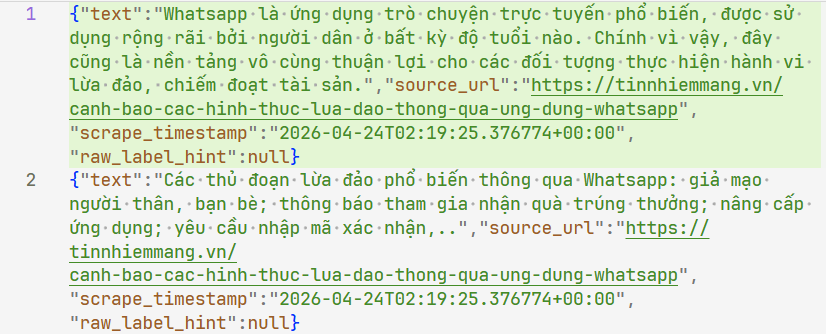
\includegraphics[width=0.92\linewidth]{figures/seed_data_sample.png}
\caption{Two rows from the retained seed file. Each row keeps the address of the advisory it came from and the time it was collected. These are public advisory texts rather than messages received by a victim; the model corpus was generated from seeds like these.}
\label{fig:seed-sample}
\end{figure}

\smallskip
\noindent\textbf{Bank impersonation (high-risk):}
\begin{quote}\small\itshape
``{[Vietcombank]} Tài khoản của bạn đã bị tạm khóa do phát hiện giao dịch bất thường. Vui lòng xác minh tại: \textup{\texttt{vcb-xacminh.vn}}''
\end{quote}

\noindent\textbf{Benign (no risk):}
\begin{quote}\small\itshape
``Techcombank: Giao dịch thành công! Tài khoản của bạn vừa nhận được 5,000,000 VND từ NGUYEN VAN AN lúc 14:32. Số dư hiện tại: 12,350,000 VND.''
\end{quote}
\smallskip

\begin{figure}[H]
\centering
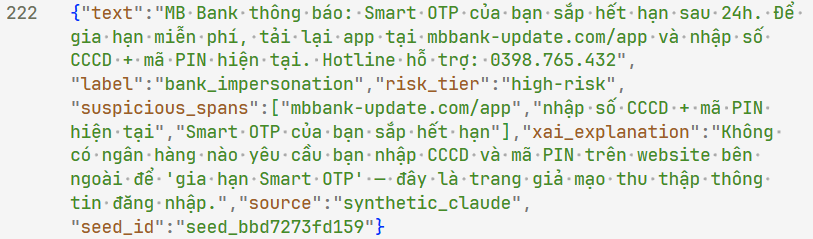
\includegraphics[width=0.92\linewidth]{figures/corpus_sample.png}
\caption{One message from the training set, showing all seven fields it carries.}
\label{fig:corpus-sample}
\end{figure}

\noindent Figure~\ref{fig:corpus-sample} shows one finished message with all of its fields filled in. The dataset was built with proper validation, but it is still not a substitute for a benchmark of real messages collected from real victims.

\noindent\textbf{Record fields:} Table~\ref{tab:record-schema} lists the seven fields every message carries. The \texttt{label} field is the one the model is graded on, it is present on every message, and it is the training target for both models.

\begin{table}[H]
\centering
\renewcommand{\arraystretch}{1.3}
\begin{tabular}{L{3.3cm}L{8.7cm}}
\toprule
\textbf{Field} & \textbf{Role} \\
\midrule
\texttt{text}              & Raw message text, natural Vietnamese with common code-switching. \\
\texttt{label}             & \textbf{Ground-truth class} for the classification task: one of \texttt{bank\_impersonation}, \texttt{zalo\_social\_engineering}, \texttt{task\_scam}, \texttt{benign}. Set during generation. \\
\texttt{risk\_tier}        & How dangerous the message is: \texttt{benign}, \texttt{suspicious}, or \texttt{high-risk}. Decided separately from the label, not calculated from it. \\
\texttt{suspicious\_spans} & The exact phrases inside \texttt{text} that justify the label: fake links, phone numbers, pressure wording. \\
\texttt{xai\_explanation}  & A short written reason for the label, which is what teaches the model to explain itself. \\
\texttt{source}            & Which model wrote the message, so every message can be traced to its generator. \\
\texttt{seed\_id}          & Links the message back to the \textit{tinnhiemmang.vn} article it was written from. Messages sharing this value always go into the same split. \\
\bottomrule
\end{tabular}
\caption{The seven fields every message in the dataset carries. Pydantic checks all of them before a message is accepted.}
\label{tab:record-schema}
\end{table}


The label is decided when the message is written, not added afterwards. Generation runs one class at a time: the prompt names the target class and states the exact JSON fields to return, so every message produced in that batch starts with that class as its label. The full prompt is in Appendix~6, together with the prompt used by the judge model and the one the finished system sends to Qwen. Building a labelled set this way is standard practice with a generative model \cite{li2024datageneration}. The review described later can drop a message or correct its label, but it does not mean every message was labelled by a person.

\noindent\textbf{Worked example:}
\begin{quote}\small\itshape
``Em đã được chọn vào suất học bổng bổ sung của trường. Để phòng tài vụ xác minh tài khoản nhận tiền, em cần chuyển phí xử lý hồ sơ học bổng hôm nay, nếu trễ suất sẽ chuyển cho bạn kế tiếp.''
\end{quote}
Its \texttt{label} is \texttt{zalo\_social\_engineering} and its \texttt{risk\_tier} is \texttt{high-risk}. Its one suspicious phrase is the exact substring ``chuyển phí xử lý hồ sơ học bổng''. The stored explanation says the message applies urgent pressure and asks for a scholarship-processing payment, which could cost the student money and expose their information.

The label is used differently by the two models. For Qwen, the label is written into the text the model has to produce, alongside the risk tier and the evidence. For PhoBERT, the label is the target of a normal four-class classification head. When a model is being scored it is given the message text only. Its answer is recorded first, and the correct label is looked up afterwards to mark that answer right or wrong, so the model can never see what it is supposed to say.

\label{sec:quality-check}
\subsection*{How quality was judged}

Three separate things check the messages, and they are not interchangeable.

The Pydantic schema check is mechanical. It confirms the required fields exist, the types are right, the label is one of the four allowed values, and the highlighted phrases are properly formed. It has no opinion about whether a message reads like a real scam.

The judge model scores meaning: how realistic the message reads, whether the label fits, how naturally Vietnamese and English are mixed, whether the risk level is right, and whether the highlighted phrases actually support the label. A message passes only if it scores at least 3 out of 5 on all five. The judge is still a model, so its verdicts are not treated as ground truth.

The human review is the only human opinion in the process. It covers a sample drawn evenly across all four classes and across both judge outcomes, so it is not just the easy messages, and it exists to check the judge rather than to replace it.

One limitation belongs with that, and it is worth following carefully because three different models are involved.

The first pass of messages was written by Claude 3.5 Haiku. The judge that scored them was a GPT-family model. For most of the set, then, the writer and the checker come from different families, which is the arrangement the check depends on.

The Zalo replacements are the exception. When that class had to be rewritten, the replacement wording was authored by a GPT-family model in a separate session, under a different prompt and a different task: rewriting a scenario into a real chat message rather than inventing one from an article. That wording was then saved into the project as fixed text and applied offline, so no API call was made during the repair itself. The result is still that, for those messages, the writer and the judge come from the same family, and the judge's verdict on them is not an independent second opinion. What all of this found is reported in Chapter~V.

\subsection*{When a correction is accepted}

The judge flagged messages whose labels looked wrong, and every one of them was reviewed by hand. Agreeing that a label is wrong is not by itself enough for the correction to be used.

The reason is the same one behind the split rule. If a hundred flagged messages all came from a single article, they are a hundred rewordings of one scenario, not a hundred separate examples of it. Accepting them together would swell one class with near-copies and make it look far more varied than it really is, which would show up as a better score without a better dataset. Corrections were therefore accepted only where they did not all trace back to one article. Applying that rule threw away a large amount of reviewed work on purpose. The counts are in Chapter~V, and Figure~\ref{fig:human-review} shows one record from the review sheet.

\begin{table}[H]
\centering
\small
\renewcommand{\arraystretch}{1.16}
\begin{tabular}{L{3.4cm}rrrrr}
\toprule
\textbf{Data split} & \textbf{Bank} & \textbf{Benign} & \textbf{Task} & \textbf{Zalo} & \textbf{Total} \\
\midrule
Training            & 595 & 517 & 306 & 240 & 1{,}658 \\
Validation          &  76 &  72 &  49 &  22 &   219 \\
Evaluation (test) &  70 &  66 &  49 &  35 &   220 \\
\midrule
\textbf{Total} & \textbf{741} & \textbf{655} & \textbf{404} & \textbf{297} & \textbf{2{,}097} \\
\bottomrule
\end{tabular}

\caption{How the 2{,}097 messages are divided between the three splits, and how many of each class each split holds.}
\label{tab:dataset-stats}
\end{table}


\begin{figure}[H]
\centering
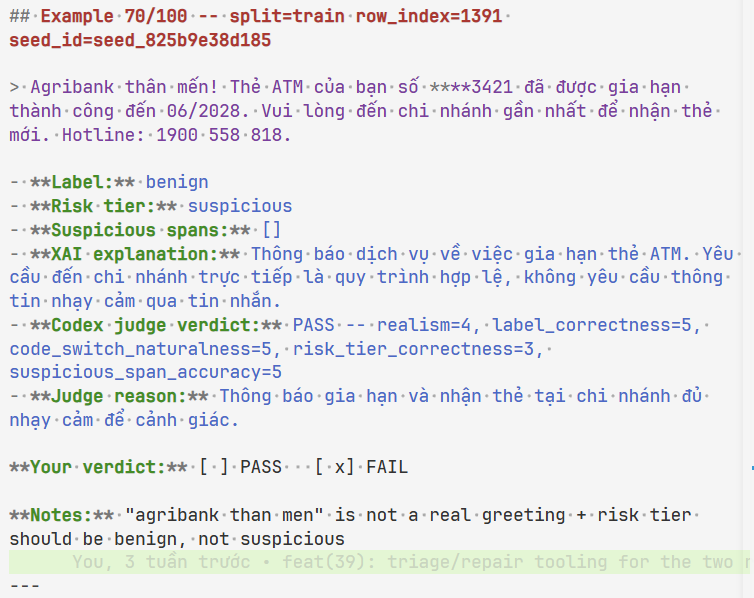
\includegraphics[width=0.92\linewidth]{figures/human_review_sheet.png}
\caption{One record from the manual review. The judge model passed it on all five scores; the reviewer disagreed, marked it FAIL, and wrote down why.}
\label{fig:human-review}
\end{figure}

\section{Offline Text Runtime Baseline}

The runtime has one text-only interface. A message comes in as text, is cleaned up locally, and is passed to whichever backend is configured. The backend returns a structured result, and a rendering layer turns it into a readable report.

Privacy is a design requirement rather than an afterthought, in line with the NIST Privacy Framework \cite{nist2026privacyframework}: the message text never leaves the device.

Before any analysis runs, the system checks that the model it is supposed to use has actually loaded. If it has not, it stops and says so rather than quietly continuing with something else. This matters more than it sounds: the project holds several models and several versions of the same model, and an answer produced by the wrong one would look exactly like a correct answer. The check names the model and the version it loaded, so a result can always be attributed to the model that produced it.

\section{Local Model Selection and Deployment Paths}

To pick a Qwen model, three models from the Qwen family \cite{qwen2025} were tested on the same 33 example messages: \texttt{qwen3-4b-instruct-2507}, \texttt{qwen3.5-4b}, and \texttt{qwen2.5-7b-instruct}. The test scored them on catching risky messages first. It used three risk levels rather than four classes --- benign, suspicious, and high-risk --- and it ran on the same laptop the real training would use, so hardware limits were part of the decision from the start.

All three caught risky messages at the same rate on this small test, so the difference came down to what each one cost in memory and time. Table~\ref{tab:pilot-comparison} gives the numbers. This was a quick screening test on 33 examples run before any fine-tuning; it picked a model that fits the laptop, and it is not a measurement of which model is better in general.

\begin{table}[H]
\centering
\resizebox{\linewidth}{!}{%
\renewcommand{\arraystretch}{1.3}
\begin{tabular}{lcccc}
\toprule
\textbf{Model tested} & \textbf{Risky messages caught} & \textbf{Peak VRAM (GB)} & \textbf{Seconds per message} & \textbf{Outcome} \\
\midrule
qwen3-4b-instruct-2507  & 0.5000 & 2.77 & 0.35 & \textbf{Chosen} \\
qwen3.5-4b              & 0.5000 & 3.28 & 0.94 & Runner-up \\
qwen2.5-7b-instruct     & 0.5000 & 5.62 & 0.56 & Too large \\
\bottomrule
\end{tabular}%
}

\smallskip
{\footnotesize Note: all three caught risky messages at the same rate, so the choice came down to memory and speed. The chosen 4B model matched the others while using less of both than the second 4B model, and the 7B model needed twice the memory. These are small-sample numbers from a screening test; they do not show that one model family is generally faster or better.}
\caption{Screening test on 33 fixed examples, 11 at each risk level, run before any fine-tuning. It picked a Qwen model that fits the laptop; it is not a result.}
\label{tab:pilot-comparison}
\end{table}


\texttt{Qwen3-4B-Instruct-2507} was chosen because it matched the others on catching risky messages, fit the laptop most comfortably, and could produce the whole structured answer.

\label{sec:qwen-vs-phobert}
PhoBERT \cite{nguyen2020phobert} was then added as a second, different kind of model rather than a second Qwen. The difference between them is the reason both are here:

\begin{itemize}\itemsep2pt
\item \textbf{Qwen} produces everything the system needs in one answer: the class label, the risk level, the suspicious phrases quoted from the message, and the written explanation.
\item \textbf{PhoBERT} produces the class label only. It is a Vietnamese encoder with a four-class head, and it has no way to generate quoted evidence or advice.
\end{itemize}

\noindent So the two models are not interchangeable. PhoBERT is a strong, compact reference point for the classification part alone, and as reported later it scores higher on that part. Qwen is the model the system actually needs, because it can also write the explanation, and the classification is only one of the four things the answer has to contain. The comparison in this thesis covers the one thing both models do.

\subsection{Whether Fine-Tuning Was Needed at All}
\label{sec:why-finetune}

Choosing a model does not answer a more basic question: whether the model needed to be trained at all, or whether a careful prompt would have been enough. That was measured rather than assumed. The chosen model was scored on the same 254 messages twice, once with prompting alone and once after QLoRA. Table~\ref{tab:finetuning-gain} gives both.

\begin{table}[H]
\centering
\small
\renewcommand{\arraystretch}{1.18}
\begin{tabular}{L{3.5cm}rrr@{\hskip 14pt}rrr}
\toprule
& \multicolumn{3}{c}{\textbf{Prompting only}} & \multicolumn{3}{c}{\textbf{After QLoRA}} \\
\cmidrule(r){2-4}\cmidrule(l){5-7}
\textbf{Class} & \textbf{Prec.} & \textbf{Recall} & \textbf{F1} & \textbf{Prec.} & \textbf{Recall} & \textbf{F1} \\
\midrule
Bank impersonation      & 0.5045 & 1.0000 & 0.6707 & 0.8615 & 1.0000 & 0.9256 \\
Zalo social engineering & 0.8806 & 0.7867 & 0.8310 & 1.0000 & 0.9867 & 0.9933 \\
Task scam               & 0.7091 & 0.6290 & 0.6667 & 1.0000 & 0.8710 & 0.9310 \\
Benign                  & 1.0000 & 0.3443 & 0.5122 & 1.0000 & 1.0000 & 1.0000 \\
\midrule
\textbf{Macro F1}       & \multicolumn{3}{c}{\textbf{0.6702}} & \multicolumn{3}{c}{\textbf{0.9625}} \\
\textbf{Accuracy}       & \multicolumn{3}{c}{\textbf{0.6890}} & \multicolumn{3}{c}{\textbf{0.9646}} \\
\bottomrule
\end{tabular}
\caption{The same base model, \texttt{Qwen3-4B-Instruct-2507}, on the same 254 messages before and after QLoRA fine-tuning. This is the earlier validation set, not the final dataset, and each column is one run.}
\label{tab:finetuning-gain}
\end{table}


\noindent Macro F1 went from 0.6702 to 0.9625. The interesting part is not the size of that gap but where it comes from. Reading down the first three columns, the model without training has perfect recall on bank impersonation and a precision of 0.5045, and on benign messages the reverse: perfect precision and a recall of 0.3443. It labelled 111 of the 254 messages as bank impersonation when only 56 of them were, and it accepted only 21 of the 61 safe messages as safe.

In other words, the untrained model was not detecting scams; it was calling almost everything a scam. That produces respectable-looking recall on the dangerous classes while making the tool useless, because a warning that fires on every message tells the user nothing. Fine-tuning is what taught the model where the boundaries are, and the largest single gain in the table is on the benign class, which is exactly the class an alarmed model gets wrong.

This measurement used the earlier 254-message validation set rather than the final dataset, and each column is a single run. It is reported as the reason this project fine-tunes rather than prompts, not as one of its results; the results are in Chapter~V.

\subsection{The Choice Between LoRA and QLoRA}
Both options were measured on the target laptop, and those measurements are reported in Chapter~IV.

The decision came down to memory rather than quality. Ordinary LoRA ran, but it left almost no video memory free and pointed at a schedule of roughly eighteen hours. No out-of-memory error occurred, and this report does not claim one did. The problem is that an eighteen-hour run with almost no memory to spare is a bad bet: any brief extra allocation would end it, and the cost of that is most of a day.

QLoRA keeps the base model frozen in 4-bit, which leaves a workable margin and cuts the step time to a few seconds. It costs little in quality, because the authors of QLoRA report that 4-bit fine-tuning reaches the quality of 16-bit fine-tuning \cite{dettmers2023qlora}. The choice was therefore about memory and risk, not about accepting a worse model.

\subsection{How Qwen Is Trained}
Each message is turned into an instruction and a JSON answer holding the label, risk tier, suspicious phrases, and explanation. Both parts are written under \texttt{Instruction} and \texttt{Response} headings, cut to at most 1{,}024 tokens, and the model is trained to produce the whole thing. The run itself is described in Chapter~IV.

\subsubsection*{Why the label is generated as text}

There are two ways to get a class decision out of a fine-tuned model.

\textbf{The traditional way} is to attach a small scoring layer to the end of the model. That layer outputs a label and nothing else. It is accurate and uses very few extra parameters \cite{yousefiramandi2025finetuning}. The problem is that it cannot write text. This project needs three outputs --- a label, a quoted piece of evidence, and a written explanation --- so a scoring layer would mean building a separate text generator as well and then trying to stitch the two outputs together afterwards.

\textbf{The approach used here} treats classification as text generation, an idea introduced with T5 \cite{raffel2020t5}. The model is trained to produce one JSON object containing all three fields at once. Three things follow from that:

\begin{itemize}\itemsep2pt
\item \textbf{One answer, one pass.} The label, the evidence, and the explanation are produced together rather than assembled from separate components.
\item \textbf{Better agreement between them.} Narang et al.\ found that generating a label together with its explanation makes the explanation match the label more closely than producing the label first and explaining it afterwards \cite{narang2020wt5}.
\item \textbf{No extra layers.} QLoRA adapts the model's existing weights, so nothing classification-specific is bolted on. The model simply learns to write one of four fixed strings: \texttt{bank\_impersonation}, \texttt{zalo\_\allowbreak social\_\allowbreak engineering}, \texttt{task\_scam}, and \texttt{benign}. That is the mechanism Schick and Sch{\"u}tze call a \textit{verbalizer} \cite{schick2021pet}.
\end{itemize}

\noindent A scoring layer would still be the better choice if a label were all that was needed, but this system also has to produce the risk tier, the quoted evidence, and the written explanation.

The adapted forward pass combines the frozen pretrained weight matrix~$W_0$ with the low-rank product~$BA$, scaled by~$\alpha/r$:
\begin{equation}
  h = W_0\, x + \frac{\alpha}{r}\, B A\, x
  \label{eq:qlora-forward}
\end{equation}
where $B \in \mathbb{R}^{d \times r}$, $A \in \mathbb{R}^{r \times k}$, and $r \ll \min(d, k)$.

\noindent\textbf{How the training run was set up:}

\begin{itemize}\itemsep2pt
\item \textbf{Memory.} The model's original weights $W_0$ stay frozen in 4-bit NF4. Only the two small added matrices $A$ and $B$ from Equation~\ref{eq:qlora-forward} are updated. This is what lets a 4B model train on a laptop.
\item \textbf{Batch size.} The model reads one instruction-and-answer pair at a time, and the weights are updated after every four of them, giving an effective batch size of 4.
\item \textbf{How it learns.} The usual next-word training loss is applied across the whole answer, including the label text itself. If the model writes the wrong label, that mistake is penalised directly, the same as any other wrong word.
\end{itemize}

\begin{table}[H]
\centering
\small
\renewcommand{\arraystretch}{1.12}
\begin{tabular}{L{5.0cm}L{8.0cm}}
\toprule
\textbf{Configuration / Result} & \textbf{Value} \\
\midrule
Base model & \texttt{Qwen3-4B-Instruct-2507} \\
Adaptation & Genuine 4-bit QLoRA; NF4 with double quantization \\
LoRA rank / scale & $r=16$, $\alpha=32$ \\
Quantized modules & 252 \texttt{Linear4bit} modules \\
Trainable adapter tensors & 504; base weights frozen \\
Random seed & 42 \\
Training / validation rows & 1{,}658 / 219 \\
Epochs / optimizer steps & 3 / 1{,}245 \\
Selected checkpoint & Step 200, chosen on the validation set \\
Validation accuracy / macro F1 & 0.9908675799 / 0.9885153110 \\
Unreadable outputs / risky called safe & 0 / 0 on validation \\
Software versions & Python 3.13.13; PyTorch 2.12.0+cu132; Transformers 5.9.0; PEFT 0.19.1; bitsandbytes 0.50.1 \\
Export & GGUF Q8\_0, 4{,}280{,}403{,}232 bytes \\
\bottomrule
\end{tabular}
\caption{The settings used for the Qwen QLoRA training run, and the score of the checkpoint that was selected. The 220 held-out messages played no part in choosing it.}
\label{tab:qlora-config}
\end{table}


Table~\ref{tab:qlora-config} lists the settings the run actually used. The two quantization settings do different jobs, and they are chosen for different reasons. NF4 is used during \textit{training}, where the goal is to fit the model into 8~GiB at all. Q8\_0 is used for the \textit{exported} file, where the goal is to run well on a CPU through \texttt{llama.cpp} \cite{gerganov2023llamacpp}. Q4 would have made the file smaller still, but a comparison of every \texttt{llama.cpp} quantization format found that Q8\_0 keeps almost all of the original quality while lower settings lose more of it \cite{kurt2026quantization}. Since the Q8\_0 file already fits comfortably on an ordinary laptop, there was nothing to gain by compressing further and accepting the extra loss.

\section{Explainable Threat Decisioning}
\label{sec:explainable-decisioning}

For each message the system returns a risk level (benign, suspicious, or high-risk), the threat label, the suspicious phrases quoted from the message itself, and a short written explanation. The explanation should be given on evidence the reader can check in the message, not on a confidence score \cite{rjoub2023surveyxai}.

Alongside those four, the runtime asks the model for a short list of safe next steps. This is the one part of the answer that the training data does not contain, because the dataset stores no such field (Table~\ref{tab:record-schema}); the model is prompted for it and the result is filtered afterwards. It is therefore reported as a runtime feature rather than as something the model learned, and no claim is made about its accuracy.

Two rules keep the whole answer honest. Quoted phrases must appear in the message text itself, and every suggested next step must stay inside a safe, generic set, so the system cannot tell a user to click a link, reply, or share a code.

\subsection*{Handling a model that writes free text}

A classification head always returns a clean result. A generative model does not: it writes free text, and nothing guarantees the JSON is well formed. The system therefore never trusts the model's raw output. It handles this in two steps.

\textbf{Step one: find and read the JSON.} The runtime scans the whole raw output for anything that could be a JSON object, scores each candidate on how well its fields match what is expected, and keeps the best one. If nothing can be read as JSON at all, it raises an error rather than guessing a label or quietly falling back to \texttt{benign}.

\textbf{Step two: check the answer makes sense.} Even valid JSON can contradict itself, because the model writes it one word at a time. Four rules are applied before anything is shown:

\begin{itemize}\itemsep2pt
\item \texttt{benign} cannot appear alongside any other threat label.
\item If the risk level is \texttt{benign}, the label must be \texttt{benign} too.
\item If the risk level is not \texttt{benign}, the label must not be \texttt{benign}.
\item If the risk level is \texttt{high-risk}, there must be at least one piece of evidence, not an empty list.
\end{itemize}

\noindent An answer that breaks any of these is rejected instead of displayed. A classification head never needs these checks, because it only ever emits one label and so cannot disagree with itself.

\section{Design Principles}

Four principles run through the whole system.

\textbf{Privacy first.} The message never leaves the device. Every later decision in the design had to keep that true.

\textbf{Honest data.} Messages written from the same article are kept together and counted as one source, so rewording a single scam cannot quietly inflate the dataset into looking more varied than it is.

\textbf{Explanations that can be checked.} The system quotes the phrases it reacted to, so a user can judge the answer instead of trusting a number.

\textbf{Missing a scam is worse than a false alarm.} A false alarm costs the user a moment of checking. A missed scam can cost them their money, so the system is tuned to prefer the first mistake over the second.
